\documentclass[10pt,conference]{IEEEtran}

\ifCLASSINFOpdf
  \usepackage[pdftex]{graphicx}
\else
\fi
\usepackage[cmex10]{amsmath}
\usepackage{amsthm,amsfonts,amssymb}
\usepackage{ifthen}
\usepackage{tikz}
\usetikzlibrary{decorations.text}
\usepackage{cite}
\usepackage{amsthm,amsfonts,amssymb}
\setcounter{MaxMatrixCols}{17}
\usepackage{graphicx}
%\usepackage[outdir=./]{epstopdf}
%\usepackage{epigraph}
%\usepackage{tikz}
%\usepackage{natbib}
%\setcitestyle{square}
\usepackage{subfig}
\usepackage{blkarray}
\usepackage{dsfont}
\usepackage[mathscr]{euscript}
\usepackage{enumitem}

\usepackage[top=1in, bottom=1in, left=1in, right=1in]{geometry}
\usepackage{amsfonts}
\usepackage{mathrsfs} 


\usepackage{algorithm}
\usepackage[noend]{algpseudocode}
\usepackage{blkarray}
\usepackage{stfloats}%
%\newtheorem{theorem}{Theorem}
\newtheorem{theorem}{Theorem}[section]
\newtheorem{corollary}{Corollary}[section]
\newtheorem{proposition}{Proposition}[section]
\newtheorem{lemma}{Lemma}[section]
\theoremstyle{remark}
\newtheorem*{remark}{Remark}
\theoremstyle{definition}
\newtheorem{definition}{Definition}[section]
\newtheorem{example}{Example}[section]
\usepackage{url}
\usepackage{tcolorbox}
\usepackage{arydshln}
\usepackage{mathtools}
\usepackage{dsfont}
\definecolor{brickred}{cmyk}{0,0.89,0.94,0.28}
\definecolor{goldenrod}{cmyk}{0,0.10,0.84,0}
\definecolor{purple}{cmyk}{0.45,0.86,0,0}
\definecolor{rawsienna}{cmyk}{0,0.72,1,0.45}
\definecolor{olivegreen}{cmyk}{0.64,0,0.95,0.40}
\definecolor{peach}{cmyk}{0,0.5,0.7,0}
\definecolor{darkolive}{rgb}{0.,0.4,0.}
\colorlet{grey}{gray!40}

\def\tcw{\textcolor{white}}
\def\tcbr{\textcolor{brickred}}
\def\tcbl{\textcolor{blue}}
\def\tcrs{\textcolor{rawsienna}}
\def\tcog{\textcolor{olivegreen}}
\def\tcpl{\textcolor{purple}}
\def\tcgr{\textcolor{grey}}

\DeclareMathOperator{\argmin}{\text{argmin}}

\global\long\def\P{\mathbb{P}}
\global\long\def\E{\mathbb{E}}
\global\long\def\V{\mathrm{Var}}
\global\long\def\C{\mathrm{Cov}}
\global\long\def\I{\mathbbm{1}}
\global\long\def\d{\mathrm{d}}

\usepackage{xcolor}
\newcommand\arv[1]{{\color{red}\textbf{Arvind: #1}}}

\usepackage{xcolor}
\newcommand\pra[1]{{\color{blue}\textbf{Prajjwal: #1}}}

\DeclarePairedDelimiter\ceil{\lceil}{\rceil}
\DeclarePairedDelimiter\floor{\lfloor}{\rfloor} % Use the [cmex10] option to ensure 
\interdisplaylinepenalty=2500

\usepackage[cmintegrals]{newtxmath}



\hyphenation{op-tical net-works semi-conduc-tor}


\begin{document}
\title{Bounding User Contributions for User-Level Differentially Private Mean Estimation}
%\author{
%\IEEEauthorblockN{V.~Arvind~Rameshwar}
%\IEEEauthorblockA{IUDX Program Unit\\IISc, Bengaluru, India\\
%	Email: arvind.rameshwar@gmail.com}
%\and
%\IEEEauthorblockN{Anshoo~Tandon}
%\IEEEauthorblockA{IUDX Program Unit\\IISc, Bengaluru, India\\
%	Email: anshoo.tandon@gmail.com}
%\and
%\IEEEauthorblockN{Abhay~Sharma}
%\IEEEauthorblockA{IUDX Program Unit\\IISc, Bengaluru, India\\
%	Email: abhay.sharma@datakaveri.org}
%}
\author{\IEEEauthorblockN{
		V.~Arvind~Rameshwar\ \
		and\ \ 
		Anshoo~Tandon
	}
	\thanks{The authors are with the India Urban Data Exchange Program Unit, Indian Institute of Science, Bengaluru, India, emails: \texttt{\{arvind.rameshwar, anshoo.tandon\}@gmail.com}.}
}
\IEEEoverridecommandlockouts
\maketitle


\begin{abstract}

We revisit the problem of releasing the sample mean of bounded samples in a dataset, privately, under user-level $\varepsilon$-differential privacy (DP). We aim to derive the optimal method of preprocessing data samples, within a canonical class of processing strategies, in terms of the error in estimation. Typical error analyses of such \emph{bounding} (or \emph{clipping}) strategies in the literature assume that the data samples are independent and identically distributed (i.i.d.), and sometimes also that all users contribute the same number of samples (data homogeneity)---assumptions that do not accurately model real-world data distributions. Our main result in this work is a precise characterization of the preprocessing strategy that gives rise to the smallest \emph{worst-case} error over all datasets -- a \emph{distribution-independent} error metric -- while allowing for data heterogeneity. We also show via experimental studies that even for i.i.d. real-valued samples, our clipping strategy performs much better, in terms of \emph{average-case} error, than the widely used bounding strategy of Amin et al. (2019).
\end{abstract}

% no keywords




% For peer review papers, you can put extra information on the cover
% page as needed:
% \ifCLASSOPTIONpeerreview
% \begin{center} \bfseries EDICS Category: 3-BBND \end{center}
% \fi
%
% For peerreview papers, this IEEEtran command inserts a page break and
% creates the second title. It will be ignored for other modes.
\IEEEpeerreviewmaketitle



\section{Introduction}
%Federated learning (FL) is now a widely studied framework for the collaborative training of a machine learning (ML) model by a large collection of devices (also called clients or users), by using decentralized training data. Typically, such a training task proceeds iteratively; in every round, each participating client performs a local update to the machine learning model using its training data and then sends this update to a central server, which is tasked with ``aggregating" the received updates. The aggregated model is then communicated back to the clients, which then begin a fresh round of local model updates. A canonical FL algorithm is the \texttt{FedAvg} algorithm introduced in \cite{fl-mcmahan}. Importantly, FL allows for the training of a large-scale ML model in a distributed fashion, while ensuring that the training data remains private to each client. For a thorough survey of the challenges in real-world deployment of FL, we refer the reader to \cite{kairouz-survey,li-survey}.

In this article, we concern ourselves with the fundamental problem of processing bounded, potentially vector-valued samples in a dataset, for the release of a private estimate of the sample mean. In particular, we work within the framework of ``user-level" differential privacy \cite{userlevel,hetero}, which is a generalization of the now widely adopted framework of differential privacy (DP) \cite{dworkroth, vadhan2017} for the design and analysis of privacy-preserving algorithms. Loosely speaking, user-level DP guarantees the privacy of a ``user", who could contribute more than one sample, by ensuring the statistical indistinguishability of outputs of the algorithm to changes in the user's samples. User-level DP has practical relevance for inference tasks on most real-world datasets, such as traffic datasets, datasets of user expenditures, and time series data, where different users contribute potentially different numbers of samples (data heterogeneity) \cite{usereg3,usereg4}. Moreover, user-level DP algorithms are increasingly becoming popular subroutines for integration into
federated learning (FL) frameworks -- see, e.g., \cite[Sec. 4]{kairouz-survey} for more details. 

%User-level privacy assumes significance in the context of real-world IoT datasets, such as traffic databases, which record multiple contributions from every user (see also \cite{usereg1,usereg2,usereg3,usereg4}). Specifically, user-level DP mechanisms for mean estimation \cite{userlevel,usereg4} are employed by the central server in a canonical FL algorithm such as \texttt{FedAvg} \cite{fl-mcmahan}, while computing a weighted average of gradients passed by each client; these mechanisms help ensure the privacy of a single user (or client), who potentially contributes several samples to the training dataset. 

There are two key requirements of such user-level DP mechanisms for mean estimation, for real-world applications. Firstly, the mechanisms must be designed to work with heterogeneous data. Secondly, one would like reliable reconstruction of the true sample mean, even when the data samples are non-i.i.d. (independent and identically distributed). Our focus is hence to  characterize an error metric, which is independent of the underlying data distribution and can be explicitly computed and optimized, for heterogeneous data.

%The second requirement is of particular importance in FL applications, where each client would like to reliably reconstruct the aggregated model update, in every round, from the noisy, privatized aggregate released by the central server, while running the FL algorithm on highly correlated real-world datasets.  

In this article, we confine our attention to (pure) $\varepsilon$-DP algorithms for mean estimation. A key subroutine in most user-level $\varepsilon$-DP mechanisms \cite{userlevel,hetero-user-level,hist-user-level,amin} is the preprocessing of the data samples for the release of an estimate of the sample mean, which requires the addition of less noise for privacy (measured via the sensitivity of the estimate), as against releasing a noised version of the true sample mean. Such a preprocessing procedure (also called a strategy for ``bounding" or ``clipping" strategy \cite{amin}) either drops certain samples contributed by selected users, or projects the samples to a ``high-probability interval" that is a strict subset of the interval in which the sample values are known to lie. While it is usually easy to establish that the mechanisms designed using the clipped estimators are differentially private, an analysis of their ``utility", or the error in estimation of the true statistic, often relies on distributional assumptions about the dataset. 

In this work, following \cite{dp_spcom,dp_preprint,tit-preprint}, we define and explicitly compute the \emph{worst-case error}, over all datasets, of general preprocessing (or bounding) strategies. The worst-case error metric is natural in settings with arbitrarily correlated data, where each user potentially ascribes his/her error tolerance to the worst dataset that the statistic is computed on. Furthermore, this error metric is clearly distribution independent and is computable under data heterogeneity too. We then explicitly identify the bounding strategy that results in the smallest worst-case error; our approach is hence an extension of those in \cite{amin} to the setting of the worst-case error, while allowing for arbitrary bounding strategies. Interestingly, we also observe from experimental studies that for scalar samples, our clipping strategy also gives rise to much smaller errors \emph{on average} compared to the strategy in \cite{amin}, for selected dataset sizes, when the samples are drawn i.i.d. according to common distributions.

%In recent work \cite{dp_spcom,dp_preprint,tit-preprint}, the authors introduced the notion of the \emph{worst-case error} incurred by a given mechanism, and showed that such an error metric is explicitly computable for selected clipped, $\varepsilon$-DP estimators for private mean and variance release. Importantly, the worst-case error metric is \emph{independent} of the distribution of the samples in the dataset, and is computable even when the data is heterogeneous. 

%In this work, we generalize the results in \cite{dp_spcom,dp_preprint} by considering clipping strategies that can project or drop data samples, potentially arbitrarily. Our analysis allows us to identify the clipping strategy that results in the smallest worst-case error -- such a strategy simply projects each data sample contributed by a user to an interval determined by the \emph{number} of samples he/she contributes. Our result can be seen as an extension of those in \cite{amin} to the setting of the worst-case error, while allowing for arbitrary bounding strategies. Interestingly, we also observe from experimental studies that our clipping strategy, which does not rely on additional, private parameter estimation unlike that in \cite{amin}, also gives rise to much smaller errors on average as compared to the strategy in \cite{amin}, for selected distributions of numbers of user contributions, when the samples are drawn i.i.d. according to common distributions.

%It is now well-understood that the release of even seemingly innocuous functions of a dataset that is not publicly available can result in the reconstruction of the identities of individuals (or users) in the dataset with alarming levels of accuracy (see, e.g.,  \cite{narayanan, sweeney}). To alleviate concerns over such attacks, the framework of differential privacy (DP) was introduced in \cite{dwork06}, which guarantees the privacy of any single sample. Subsequently, several works (see the surveys \cite{dworkroth, vadhan2017} for references) have designed DP mechanisms for the release of statistics such as the mean, variance, and histograms.




\section{Notation and Preliminaries}
\section{Preliminary}

\paragraph{Notation} Consider a sentence of $T$ tokens $\vx=\{\vx_1,\ldots, \vx_T\}\in\gX$, and let $P$ be the unknown target language distribution, $\tilde P(\vx)$ be the empirical distribution of the training data (which is an approximation of $P$), and $Q$ be the distribution of our model at hand. Since our paper is also closely related to RLHF, we will also use $\pi$ to represent the distributions. In particular, we sometimes write $\pi_\theta$ for a distribution that is parameterized by $\theta$, where $\theta$ is usually the set of trainable parameters of the LLM; we write $\pr$ for a reference distribution that should be clear given the context. The next token prediction loss is minimizing the forward-KL between $P$ and $Q$. 




\section{Worst-Case Errors of Bounding Strategies}
\label{sec:bound}
%In this section, we present an explicit characterization of the worst-case errors for a broad class of strategies that work by ``bounding" or ``clipping" the contributions of users, as mentioned in the Introduction. In other words, the estimator $\overline{f}$ of $f$ in \eqref{eq:Mbar} is a suitably clipped or bounded version of the sample mean $f$. We then identify that clipping strategy that leads to the smallest worst-case error.
\subsection{On Clipping Strategies}
We work with estimators $\overline{f} = \overline{f}_{\left\{a_j^{(\ell)},b_j^{(\ell)}\right\}}$ of $f$ obtained by bounding user contributions as follows: for each $\ell\in [L]$ and $j\in [m_\ell]$, we let $\overline{\mathbf{x}}_j^{(\ell)}:= {\mathsf{A}_{a_j^{(\ell)},b_j^{(\ell)}}}\left(\mathbf{x}_j^{(\ell)}\right)$, for reals $0\leq a_j^{(\ell)}\leq b_j^{(\ell)}\leq U$. In words, $\overline{\mathbf{x}}_j^{(\ell)}$ is a projection of $\mathbf{x}_j^{(\ell)}$ onto the set $\mathsf{A}_{a_j^{(\ell)},b_j^{(\ell)}}$, which, intuitively, reduces the range of values that $\mathbf{x}_j^{(\ell)}$ can take, and hence its sensitivity too. Figure \ref{fig:proj} shows a pictorial depiction of the annulus $\mathsf{A}_{a_j^{(\ell)},b_j^{(\ell)}}$ when $d=2$ and examples of projections onto the annulus. We then set 
$
\overline{f} = \overline{f}(\mathcal{D}):= \frac{1}{\sum_{\ell'=1}^L m_{\ell'}}\cdot \sum_{\ell=1}^L \sum_{j=1}^{m_\ell} \mathbf{\overline{x}}_j^{(\ell)}.
$
\begin{figure}
	\centering
	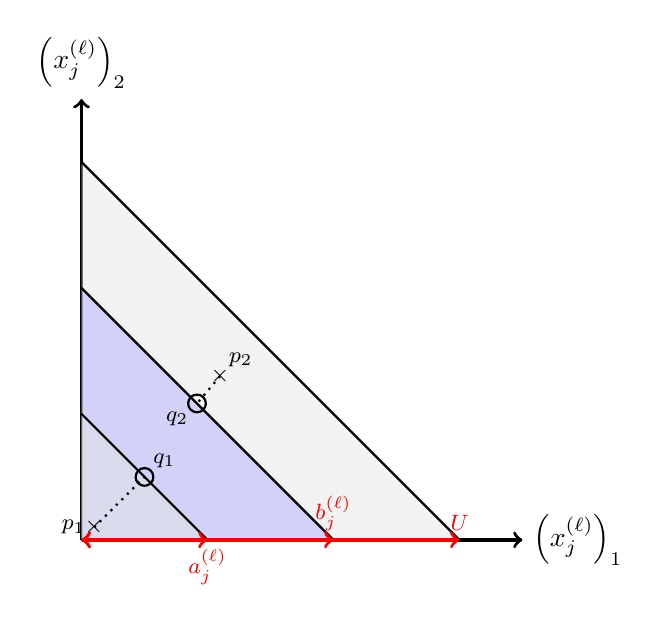
\begin{tikzpicture} [scale=1.6]% Adjust scale as needed
		
		\newcommand{\outerradius}{3}
		\newcommand{\middleradius}{2}
		\newcommand{\innerradius}{1}
		
		% Draw the axes with new labels (only positive quadrant)
		\draw[->, very thick] (0,0) -- (\outerradius+0.5,0) node[right] {$\left(x_j^{(\ell)}\right)_1$};
		\draw[->, very thick] (0,0) -- (0,\outerradius+0.5) node[above] {$\left(x_j^{(\ell)}\right)_2$};
		
		% Draw the balls with transparency (only positive quadrant)
		\draw[thick, fill=gray!20, fill opacity=0.5] (0,\outerradius) -- (\outerradius,0) -- (0,0);
		
		% Draw the blue region *first* (only positive quadrant)
		\fill[blue!30, fill opacity=0.5] (0,\middleradius) -- (\middleradius,0) -- (0,0);
		
		% Draw the inner ball - make it transparent gray (only positive quadrant)
		\draw[thick, fill=gray!20, fill opacity=0.5] (0,\innerradius) -- (\innerradius,0) -- (0,0); % Inner ball
		
		% Draw the middle ball outline in BLACK (only positive quadrant)
		\draw[thick,black] (0,\middleradius) -- (\middleradius,0) -- (0,0);
		
		\footnotesize
		% Add arrows and labels (red, bold tips)
		\draw[<->, very thick, red, line cap=round] (0,0) -- (\innerradius,0) node [below,font=\footnotesize] {$a_j^{(\ell)}$};
		\draw[<->, very thick, red, line cap=round] (0,0) -- (\middleradius,0) node [above,font=\footnotesize] {$b_j^{(\ell)}$};
		
		\draw[<->,very thick, red, line cap=triangle] (0,0) -- (\outerradius,0) node [above,font=\footnotesize] {$U$};
		
		% Mark the point (0.1, 0.1) and line segment
		\draw[thick, black] (0.1,0.1) node {\textbf{$\times$}} node[left] {$p_1$};
		\draw[dotted, thick] (0.1,0.1) -- (0.5,0.5);
		
		% Calculate the endpoint of the second line segment
		\pgfmathsetmacro{\endx}{1.1/1.2}
		\pgfmathsetmacro{\endy}{1.3/1.2}
		
		% Mark the point (1.1, 1.3)/1.2 with a circle
		\draw[thick, black] (\endx,\endy) circle (2pt) node[below left]{$q_2$};
		
		% Mark the point (1.1, 1.3)
		\draw[thick, black] (1.1,1.3) node {\textbf{$\times$}} node[above right]{$p_2$};
		
		% Draw the dotted line segment from (1.1, 1.3)
		\draw[dotted, thick] (1.1,1.3) -- (\endx,\endy);
		
		% Mark the point (0.5, 0.5) with a circle
		\draw[thick, black] (0.5, 0.5) circle (2pt) node[above right]{$q_1$};
		
	\end{tikzpicture}
	\caption{The annulus $\mathsf{A}_{a_j^{(\ell)},b_j^{(\ell)}}$, for $d=2$, shown in blue. Here, the points $q_1$, $q_2$ equal $\mathsf{A}_{a_j^{(\ell)},b_j^{(\ell)}}(p_1)$ and $\mathsf{A}_{a_j^{(\ell)},b_j^{(\ell)}}(p_2)$, respectively.}
	\label{fig:proj}
\end{figure}
Note that the class $\mathsf{B}$ of estimators $\overline{f}$ as above  captures those estimators obtained by dropping selected samples $\mathbf{x}_j^{(\ell)}$ (by setting $a_j^{(\ell)}= b_j^{(\ell)} = 0$ for those samples) and those obtained by projecting samples onto an $\ell_1$-bounded subset of $\Delta_U$, in addition to strategies that perform a combination of dropping and projection. This class of estimators hence includes several common estimators of the sample mean used in works such as \cite{userlevel,dp_preprint,tit-preprint}.

%In the next subsection, we discuss the worst-case errors (as in \eqref{eq:eg}) of mechanisms that employ some $\overline{f}\in \mathsf{B}$ as the estimator of the sample mean.

\subsection{On Worst-Case Errors of Clipping Strategies}
\label{sec:worst-case}
Consider the quantity $E_{\overline{f}}$, for $\overline{f}\in \mathsf{B}$. The following proposition then holds:
\begin{proposition}
	\label{lem:worst-case}
	We have that
	\begin{align*}
		E_{\overline{f}} \notag&= \frac{1}{\sum_{\ell'\leq L} m_{\ell'}}\cdot \left(\sum_{\ell\leq L}\sum_{j\leq m_\ell} \max\left\{a_j^{(\ell)},U-b_j^{(\ell)}\right\}\right)\ + \notag\\
		&\ \ \  \ \ \ \ \ \ \  \ \ \ \ \ \ \ \  \ \ \ \  \ \ \ \frac{d\cdot\max_{\ell\leq L} \sum_{j\leq m_\ell} \left(b_j^{(\ell)}-a_j^{(\ell)}\right)}{\varepsilon\cdot \sum_{\ell'\leq L} m_{\ell'}}.
	\end{align*}
\end{proposition}
The proof of Proposition \ref{lem:worst-case} proceeds with help from a few lemmas. For $E_{\overline{f}}$ as in \eqref{eq:eg}, we define $\beta(\overline{f})$ to be the bias, i.e., $\beta(\overline{f}):= \max_{\mathcal{D}\in \mathsf{D}} \big \lVert f(\mathcal{D}) - \overline{f}(\mathcal{D}) \big\rVert$ and $\eta(\overline{f})$ to be the error due to noise addition, i.e., $\eta(\overline{f}):= \E[\lVert\mathbf{\mathbf{Z}}\rVert_1]$. First, we aim to characterize $\beta(\overline{f})$. To this end, we first state a necessary condition for a vector $\mathbf{y}$ to be an $\ell_1$-projection of a vector $\mathbf{a}\in \Delta_U$ onto $\Delta_\alpha$, for $ \alpha\leq U$. 
\begin{lemma}
	\label{lem:proj1}
	Given $\mathbf{a}\in \Delta_U$ and $\alpha\leq U$, we have $\Delta_\alpha(\mathbf{a}) = \mathbf{a}$, if $\mathbf{a}\in \Delta_{\alpha}$. Else, any $\ell_1$-projection $\mathbf{y} = \Delta_\alpha(\mathbf{a})$ must satisfy $\lVert \mathbf{y}\rVert_1 = \alpha$, with $y_i\leq a_i$, for all $i\in [d]$.
\end{lemma}
\begin{proof}
	The first statement in the lemma is clear. Now, for $\mathbf{a}\notin \Delta_\alpha$, suppose that $\mathbf{y} = \Delta_\alpha(\mathbf{a})$ is such that $\lVert \mathbf{y}\rVert_1 < \alpha$. It can then be seen that by setting $\mathbf{y}':= \lambda\mathbf{y}+(1-\lambda)\mathbf{a}$, for some $\lambda\in (0,1)$ such that $\lVert \mathbf{y}'\rVert_1 = \alpha$, we will obtain that $\lVert \mathbf{y}'-\mathbf{a}\rVert_1 < \lVert \mathbf{y}-\mathbf{a}\rVert_1$, which is a contradiction. Likewise, suppose that $y_i>a_i$, for some $i\in [d]$. Now, consider any coordinate $j\in [d]$ such that $y_j\leq a_j$ (such a coordinate must exist, since $\lVert \mathbf{y}\rVert_1 = \alpha$); by letting $m:= \min\{|y_i-a_i|,|y_j-a_j|\}$ and setting $y_i \gets y_i-m$ and $y_j \gets y_j+m$, we see that we strictly decrease $\lVert \mathbf{y}-\mathbf{a}\rVert_1$, which is a contradiction.
\end{proof}
In the appendix, we explicitly characterize the vectors $\mathbf{y}\in \Delta_\alpha$ that are the $\ell_1$-projections of $\mathbf{a}\in \Delta_U\setminus \Delta_\alpha$, for $\alpha\leq U$; indeed, we have that the condition stated in Lemma \ref{lem:proj1} is both necessary and sufficient. The next lemma exactly characterizes $\beta(\overline{f})$.
\begin{lemma}
	\label{lem:proj2}
	We have that $\beta(\overline{f}) = \frac{1}{\sum_{\ell'\leq L} m_{\ell'}}\cdot \left(\sum_{\ell\leq L}\sum_{j\leq m_\ell} \max\left\{a_j^{(\ell)},U-b_j^{(\ell)}\right\}\right)$.
\end{lemma}
\begin{proof}
	For a sample $\mathbf{x}_j^{(\ell)}\in \mathsf{A}_{a_j^{(\ell)},b_j^{(\ell)}}$, it is clear that $\mathsf{A}_{a_j^{(\ell)},b_j^{(\ell)}}(\mathbf{x}_j^{(\ell)}) = \mathbf{x}_j^{(\ell)}$. Now, suppose that $\mathbf{x}_j^{(\ell)}\in \Delta_U\setminus \Delta_{b_j^{(\ell)}}$. Following Lemma \ref{lem:proj1}, if $\mathbf{y} = \mathsf{A}_{a_j^{(\ell)},b_j^{(\ell)}}(\mathbf{a})$, we must have $\lVert \mathbf{y} - \mathbf{x}_j^{(\ell)}\rVert_1 = \sum_{i\leq d} ((x_j^{(\ell)})_i - y_i) = \lVert \mathbf{x}_j^{(\ell)}\rVert_1 - b_j^{(\ell)}.$ Hence, the worst-case clipping error for sample $\mathbf{x}_j^{(\ell)}$ is $\max\ \lVert \mathsf{A}_{a_j^{(\ell)},b_j^{(\ell)}}(\mathbf{x}_j^{(\ell)}) - \mathbf{x}_j^{(\ell)}\rVert_1 = U-b_j^{(\ell)}$. By symmetric arguments, one can show that if $\mathbf{x}_j^{(\ell)}\in \Delta_{a_j^{(\ell)}}\setminus \delta_{a_j^{(\ell)}}$, we must have $\max\ \lVert \mathsf{A}_{a_j^{(\ell)},b_j^{(\ell)}}(\mathbf{x}_j^{(\ell)}) - \mathbf{x}_j^{(\ell)}\rVert_1 = a_j^{(\ell)}$. Thus, overall, we obtain that 
	\begin{equation}\max_{\mathbf{x}_j^{(\ell)}\in \Delta_U} \lVert \mathsf{A}_{a_j^{(\ell)},b_j^{(\ell)}}(\mathbf{x}_j^{(\ell)}) - \mathbf{x}_j^{(\ell)}\rVert_1 = \max\left\{a_j^{(\ell)},U-b_j^{(\ell)}\right\}. \label{eq:maxclip}\end{equation} 
	Now, for any dataset $\mathcal{D}$, recall that
	\begin{align}
		&\lVert f(\mathcal{D})-\overline{f}(\mathcal{D})\rVert_1 \notag\\
		%&=\frac{1}{\sum_{\ell'\leq L} m_{\ell'}}\left\lVert \sum_{\ell\leq L}\sum_{j\leq m_\ell} \left(\mathbf{x}_j^{(\ell)} - \overline{\mathbf{x}}_j^{(\ell)}\right)\right \rVert_1 \notag\\
		&=\frac{1}{\sum_{\ell'\leq L} m_{\ell'}}\left\lVert \sum_{\ell\leq L}\sum_{j\leq m_\ell} \left(\mathbf{x}_j^{(\ell)} - \mathsf{A}_{a_j^{(\ell)},b_j^{(\ell)}}(\mathbf{x}_j^{(\ell)}) \right)\right \rVert_1. \label{eq:cliphelp}
	\end{align}
	Putting together \eqref{eq:maxclip} and \eqref{eq:cliphelp} concludes the proof.
%	It is then easy to see that the bias
%	\begin{align}
%		&\max_{\mathcal{D}\in \mathsf{D}} |f(\mathcal{D})-\overline{f}(\mathcal{D})| \notag\\&= \frac{1}{\sum_{\ell'\leq L} m_{\ell'}}\cdot \left(\sum_{\ell\leq L}\sum_{j\leq m_\ell} \max\left\{a_j^{(\ell)},U-b_j^{(\ell)}\right\}\right). \label{eq:bias}
%	\end{align}
\end{proof}
The calculation of $\eta(\overline{f})$ is quite similar to the proof above, and is captured in Lemma \ref{lem:proj3} below.

\begin{lemma}
	\label{lem:proj3}
	We have that $\eta(\overline{f}) = \frac{d\cdot \max_{\ell\leq L} \sum_{j\leq m_\ell} \left(b_j^{(\ell)}-a_j^{(\ell)}\right)}{\varepsilon\cdot \sum_{\ell'\leq L} m_{\ell'}}.$
\end{lemma}
\begin{proof}
Via arguments entirely analogous to that in the proof of Lemma \ref{lem:proj2}, the user-level sensitivity of $\overline{f}$ is
$
	\Delta_{\overline{f}} = \frac{\max_{\ell\leq L} \sum_{j\leq m_\ell} \left(b_j^{(\ell)}-a_j^{(\ell)}\right)}{\sum_{\ell'\leq L} m_{\ell'}},
$
since in the worst-case, all samples of a user $\ell$ are changed each from $(a_j^{(\ell)},0,\ldots,0)$ to $(b_j^{(\ell)},0,\ldots,0)$. Using $\E[\lVert \mathbf{Z}\rVert_1] = d\E[|Z_1|] = d\Delta_{\overline{f}} /\varepsilon$ gives us the required result.
\end{proof}
The proof of Proposition \ref{lem:worst-case} then follows directly by putting together Lemmas \ref{lem:proj2} and \ref{lem:proj3}.
%\begin{remark}
%	Via the proof of Lemma \ref{lem:worst-case}, we observe that for a given distribution $\{m_\ell:\ell\in [L]\}$ of user contributions, the dataset $\mathcal{D}$ that gives rise to the largest (or worst-case) error is that where $x_j^{(\ell)} = U$, for all $\ell\in [L]$, $j\in [m_\ell]$. We shall use this observation in the next section when we numerically evaluate the performance of the clipping strategy in \cite{amin} on this ``worst-case dataset".
%\end{remark}


Given the characterization of the worst-case error $E_{\overline{f}}$ as above, we proceed with identifying an estimator $f^\star \in \mathsf{B}$ (equivalently, a bounding strategy) that minimizes $E_{\overline{f}}$, over all $\overline{f}\in \mathsf{B}$. Let $T_\varepsilon$ denote the $\left \lceil \left(\frac{2d}{\varepsilon}\right)\right \rceil^{\text{th}}$-largest value in the collection $\{Um_1,Um_2,\ldots,Um_L\}$; if $\varepsilon<2d/L$, we set $T_\varepsilon = 0$. Our main result is encapsulated in the following theorem:
\begin{theorem}
	\label{thm:opt}
	We have that $f^\star = \overline{f}_{\left\{a_j^{(\ell)},b_j^{(\ell)}\right\}}$ minimizes $E_{\overline{f}}$, where
	$
	a_j^{(\ell)} = \max\left\{\frac{Um_\ell-T_\varepsilon}{2m_\ell},0\right\}\text{ and } b_j^{(\ell)} = \min\left\{\frac{Um_\ell+T_\varepsilon}{2m_\ell},U\right\},
	$
	for all $\ell\in [L]$ and $j\in [m_\ell]$.
\end{theorem}
Some remarks are in order. First, note that the optimal bounding strategy $f^\star$ clips sample values based only on the number of contributions of each user $\ell\in [L]$. Furthermore, note that the interval of projection is determined by $T_\varepsilon$, which is quite similar in structure to the optimal clipping threshold $T$ in \cite{amin} for item-level DP, which is the (privately estimated) $\left \lceil \left(\frac{2}{\varepsilon}\right)\right \rceil^{\text{th}}$-largest \emph{sample value}.

The proof of Theorem \ref{thm:opt} proceeds with help from the following lemma.
\begin{lemma}
	\label{lem:helper}
	There exists an estimator $\overline{f}_{\left\{a_j^{(\ell)},b_j^{(\ell)}\right\}}$ minimizing $E_{\overline{f}}$, which obeys $a_j^{(\ell)}+b_j^{(\ell)} = U$, for all $\ell\in [L]$ and $j\in [m_\ell]$.
\end{lemma}
\begin{proof}
	Consider any optimal estimator $\overline{f}_{\left\{a_j^{(\ell)},b_j^{(\ell)}\right\}}$, and suppose that $a_j^{(\tilde{\ell})}+b_j^{(\tilde{\ell})}>U$, for some $\tilde{\ell}\in [L]$ and $j\in [m_{\tilde{\ell}}]$. The proof when we suppose that $a_j^{(\tilde{\ell})}+b_j^{(\tilde{\ell})}<U$, for some $\tilde{\ell}\in [L]$ and $j\in [m_{\tilde{\ell}}]$, is similar, and is omitted. Let $\delta =  (a_j^{(\tilde{\ell})}+b_j^{(\tilde{\ell})})-U$. By setting $b_j^{(\tilde{\ell})}\gets b_j^{(\tilde{\ell})}-\delta$, we observe that $\beta(\overline{f})$ remains unchanged, while $\eta(\overline{f})$ either remains unchanged or strictly decreases by $\delta>0$.
\end{proof}
Hence, to obtain the explicit structure of an estimator $\overline{f}$ that minimizes $E_{\overline{f}}$, it suffices to focus estimators $\overline{f}_{\left\{a_j^{(\ell)},b_j^{(\ell)}\right\}}$ with $a_j^{(\ell)}+b_j^{(\ell)} = U$, for all $\ell\in [L]$, $j\in [m_\ell]$. For $\ell\in [L]$, let $S^{(\ell)}:= \sum_{j\leq m_\ell} a_j^{(\ell)}$, for any given estimator $\overline{f}$. Then, there exists an estimator $f^\star$ minimizing $E_{\overline{f}}$ that satisfies
\begin{equation}
	\label{eq:optsimp}
	E_{f^\star} = \frac{1}{\sum_{\ell'\leq L} m_{\ell'}}\cdot \left(\sum_{\ell\leq L} S^{(\ell)}+\frac{d}{\varepsilon}\cdot \max_{\ell\leq L} \left(Um_\ell - 2S^{(\ell)}\right)\right).
\end{equation}
We now prove Theorem \ref{thm:opt}.

\begin{proof}[Proof of Thm. \ref{thm:opt}]
	We begin with the expression in \eqref{eq:optsimp}; note that our task now is simply to identify the optimal parameters $\{S^{(\ell)}:\ \ell\in [L]\}$ of $f^\star$ in \eqref{eq:optsimp}. Once these parameters are derived, we simply set $a_j^{(\ell)}:= S^{(\ell)}/m_\ell = U-b_j^{(\ell)}$ (via Lemma \ref{lem:helper}), for each $\ell\in [L]$ and $j\in [m_\ell]$. In the expression in \eqref{eq:optsimp}, let us set $\tau:= \max_{\ell\leq L} \left(Um_\ell - 2S^{(\ell)}\right)$. We hence need to solve the following constrained optimization problem:
	\begin{align}
		&{\text{minimize}}\quad h(\{S^{(\ell)}\}):= \left(\sum_{\ell\leq L} S^{(\ell)}+\frac{d\tau}{\varepsilon}\right)\notag\\
		&\text{subj. to:}\ \  Um_\ell-2S^{(\ell)}\leq \tau,\ S^{(\ell)}\geq 0,\ \forall\ \ell\in [L],\ \tau\geq 0.\label{eq:opt}
	%	&\ \ \ \  \ \ \ \  \ \ \ \ \ \ S\geq 0. \label{eq:opt}
	\end{align}
The optimization problem in \eqref{eq:opt} is a linear programming problem. By standard arguments via the necessity of the KKT conditions \cite[Sec. 5.5.3]{boyd}, there must exist reals $\lambda_\tau\geq 0$ and $\lambda_\ell,\ \mu_\ell\geq 0$, for each $\ell\in [L]$ (or Lagrange multipliers), such that the function $\mathcal{L}(\{S^{(\ell)}\},\ \lambda_\tau,\{\lambda_\ell,\mu_\ell\}):= \sum_{\ell\leq L} S^{(\ell)}+\frac{d\tau}{\varepsilon}-\lambda_\tau \tau\ + \\
\sum_\ell \lambda_\ell\cdot \left(Um_\ell-2S^{(\ell)}-\tau\right)-\sum_\ell \mu_\ell S^{(\ell)}$
%\begin{align*}
%\mathcal{L}(\{S^{(\ell)}\},\ &\lambda_S,\{\lambda_\ell,\mu_\ell\}):= \sum_{\ell\leq L} S^{(\ell)}+\frac{S}{\varepsilon}-\lambda_S S\ + \\
%&\sum_\ell \lambda_\ell\cdot \left(Um_\ell-2S^{(\ell)}-S\right)-\sum_\ell \mu_\ell S^{(\ell)}
%\end{align*}
obeys the following properties.
\begin{itemize}
	\item \textbf{Stationarity}: We have that $\frac{\partial \mathcal{L}}{\partial \tau} = 0$, or $\lambda_\tau+\sum_\ell \lambda_\ell = \frac{d}{\varepsilon},$
%	\begin{equation}
%		\label{eq:stat1}
%		\lambda_S+\sum_\ell \lambda_\ell = \frac{1}{\varepsilon},
%	\end{equation}
and that $\frac{\partial \mathcal{L}}{\partial S^{(\ell)}} = 0$, for each $\ell\in [L]$, or $\lambda_\ell = \frac{1-\mu_\ell}{2}.$
%\begin{equation}
%	\label{eq:stat2}
%	\lambda_\ell = \frac{1-\mu_\ell}{2}.
%\end{equation}
\item \textbf{Complementary slackness}: We have that $	\lambda_\tau \tau= 0,\ \lambda_\ell\cdot \left(Um_\ell-2S^{(\ell)}-\tau\right) = 0,\ \text{and}\ \mu_\ell S^{(\ell)} = 0,$
%\begin{align}
%	\label{eq:comp}
%	\lambda_SS = 0,\ \lambda_\ell\cdot \left(Um_\ell-2S^{(\ell)}-S\right) = 0,\ \text{and}\ \mu_\ell S^{(\ell)} = 0,
%\end{align}
for all $\ell\in [L]$.
\end{itemize}
We claim that the assignment $\tau^\star = T_\varepsilon$ and $S^{(\ell),\star} = \max\left\{\frac{Um_\ell-T_\varepsilon}{2},0\right\}$ satisfies the conditions above, for an appropriate choice of $\lambda_\tau,\{\lambda_\ell,\mu_\ell\}$ values. Indeed, for $\ell\in [L]$, if $S^{(\ell),\star} = 0$, we set $\lambda_\ell = 0$ and $\mu_\ell = 1$; else, we set $\lambda_\ell = \frac12$ and $\mu_\ell = 0$. 
%An optimal choice of parameters $\{a_j^{(\ell)},b_j^{(\ell)}\}$ of an estimator $f^\star$ thus obeys $a_j^{(\ell)}:= \alpha^{(\ell),\star}/m_\ell = U-b_j^{(\ell)}$, for each $\ell\in [L]$ and $j\in [m_\ell]$.
\end{proof}
Observe that from Theorem \ref{thm:opt} and \eqref{eq:optsimp}, the optimal worst-case error is $E^\text{OPT}(\varepsilon)= \frac{1}{\sum_{\ell'\leq L} m_{\ell'}}\cdot\left(\sum_{\ell\leq L} \max\left\{{Um_\ell-T_\varepsilon},0\right\}+\frac{dT_\varepsilon}{\varepsilon}\right).$ %
%\begin{align}
%&E^\text{OPT}(\varepsilon) \notag\\ &= \frac{1}{\sum_{\ell'\leq L} m_{\ell'}}\cdot\left(\sum_{\ell\leq L} \max\left\{\frac{Um_\ell-T_\varepsilon}{2m_\ell},0\right\}+\frac{1}{\varepsilon}\cdot \min_{\ell\leq L} \{T_\varepsilon,Um_\ell\}\right). \label{eq:erropt}
%\end{align}
Note that $T_\varepsilon$ is non-decreasing with $\varepsilon$. The following lemma then holds.
\begin{lemma}
\label{lem:monotonicity}
$E^\text{OPT}(\varepsilon)$ is decreasing with $\varepsilon>0$.
\end{lemma}
\begin{proof}
	Since $T_\varepsilon = Um^\star$, for all $\varepsilon\geq 2d/L$, it can be seen that $E^\text{OPT}(\varepsilon)$ is indeed non-increasing for $\varepsilon\geq 2d/L$.
	
	Now, consider $0<\varepsilon_1<\varepsilon_2<2d/L$; assume for simplicity that we have $m_1\geq m_2\geq \ldots\geq m_L$. Consider the function $g(\varepsilon,t):= \frac{1}{\sum_{\ell'\leq L} m_{\ell'}}\cdot\left(\sum_{\ell\leq L} \max\left\{{Um_\ell-t},0\right\}+\frac{dt}{\varepsilon}\right).$ Then,
	\begin{align*}
		E^\text{OPT}(\varepsilon_2)&= g\left(\varepsilon_2,Um_{\left \lceil \left(\frac{2d}{\varepsilon_2}\right)\right \rceil}\right)\\
		&\leq g\left(\varepsilon_2,Um_{\left \lceil \left(\frac{2d}{\varepsilon_1}\right)\right \rceil}\right)\\
		&< g\left(\varepsilon_1,Um_{\left \lceil \left(\frac{2d}{\varepsilon_1}\right)\right \rceil}\right) = E^\text{OPT}(\varepsilon_1),
	\end{align*}
where the first inequality holds since $t = Um_{\left \lceil \left(\frac{2d}{\varepsilon_2}\right)\right \rceil}$ minimizes $g(\varepsilon_2,t)$, over admissible values of $t$, and the second inequality holds since $\varepsilon_1<\varepsilon_2$.
\end{proof}
%Hence, we obtain that  $E^\text{OPT}(\varepsilon)$ is monotonically non-increasing as a function of $\varepsilon>0$.

A special case of Theorem \ref{thm:opt} is when $d=1$, with the interpretation that each sample $x_j^{(\ell)}\in [0,U]$. Here, the annulus $\mathsf{A}_{a_j^{(\ell)},b_j^{(\ell)}}$ is simply the interval $[a_j^{(\ell)}, b_j^{(\ell)}]\subseteq [0,U]$. This implies that for the case when the samples $\mathbf{x}_j^{(\ell)}$ are allowed to take values in the cube $[0,U]^d$, as against in the $\ell_1$-ball $\lVert \mathbf{x}_j^{(\ell)}\rVert_1\leq U$, one can perform the bounding procedure, using the \emph{same} interval $[a_j^{(\ell)}, b_j^{(\ell)}]$ identified via Theorem \ref{thm:opt} for the $d=1$ setting, for each dimension, independently.
	
%
%	\begin{figure}
%		\centering
%		\begin{tikzpicture} [scale=0.8]% Adjust scale as needed
%			
%			\newcommand{\outerradius}{3}
%			\newcommand{\middleradius}{2}
%			\newcommand{\innerradius}{1}
%			
%			% Draw the axes with new labels
%			\draw[->] (-\outerradius-1,0) -- (\outerradius+1,0) node[right] {$(x_j^{(\ell)})_1$};
%			\draw[->] (0,-\outerradius-1) -- (0,\outerradius+1) node[above] {$(x_j^{(\ell)})_2$};
%			
%			% Draw the balls with transparency
%			\draw[thick, fill=gray!20, fill opacity=0.5] (0,\outerradius) -- (\outerradius,0) -- (0,-\outerradius) -- (-\outerradius,0) -- cycle;
%			
%			% Draw the blue region *first*
%			\fill[blue!30, fill opacity=0.5] (0,\middleradius) -- (\middleradius,0) -- (0,-\middleradius) -- (-\middleradius,0) -- cycle;
%	%		\fill[white] (0,\innerradius) -- (\innerradius,0) -- (0,-\innerradius) -- (-\innerradius,0) -- cycle; % "Cut out" the inner part
%			
%			% Draw the inner ball - make it transparent gray
%			\draw[thick, fill=gray!20, fill opacity=0.5] (0,\innerradius) -- (\innerradius,0) -- (0,-\innerradius) -- (-\innerradius,0) -- cycle; % Inner ball
%			
%			% Draw the middle ball outline in BLACK
%			\draw[thick,black] (0,\middleradius) -- (\middleradius,0) -- (0,-\middleradius) -- (-\middleradius,0) -- cycle;
%			
%			\footnotesize
%			% Add arrows and labels (red, bold tips)
%			\draw[<->, very thick, red, line cap=round] (0,0) -- (\innerradius,0) node [below,font=\footnotesize] {$a_j^{(\ell)}$};
%			\draw[<->, very thick, red, line cap=round] (0,0) -- (\middleradius,0) node [above,font=\footnotesize] {$b_j^{(\ell)}$};
%			
%			\draw[<->,very thick, red, line cap=triangle] (0,0) -- (\outerradius,0) node [above,font=\footnotesize] {$U$};
%			
%			
%		\end{tikzpicture}
%		\caption{The annulus is shown in blue.}
%	\end{figure}


\section{Numerical Experiments}
\section{Experiments: Planning outperforms Heuristics}
\label{sec:experiment}

We begin our empirical demonstrations by showcasing the effectiveness of our planning framework on both synthetic and real datasets. We focus on the simplest planning algorithm, 1-step lookaheads (Algorithm~\ref{alg:complete}), and show that even basic planning can hold great promise. 
We illustrate our framework using two uncertainty quantification modules---GPs and 
\ensembles/ \ensembleplus. 

Throughout this section, we focus on evaluating the mean squared error of 
a regression model $\model$,  and develop adaptive policies that minimize uncertainty on $g(f)$ defined in~\eqref{eqn:l2-g-f}.
When GPs provide a valid model of uncertainty, 
our experiments show that our planning framework significantly outperforms other baselines. 
We further demonstrate that our conceptual framework extends to deep learning-based uncertainty quantification methods such as  \ensembleplus while highlighting computational challenges that need to be resolved in order to scale our ideas. 
For simplicity, we assume a naive predictor, i.e., $\psi(\cdot) \equiv 0$. However, we emphasize that this problem is just as complex as if we were using a sophisticated model $\psi(.)$. The performance gap between the algorithms 
primarily depends
on the level  of uncertainty in our prior beliefs.

To evaluate the performance of our algorithm, we benchmark it against several baselines. 
%Active learning baselines use an acquisition function $\ac$ to select points that have the highest   function value: $X\opt_t \in \argmax_{X \in \xpoolj{t}} \ac({X})$ at every step $t$. These methods may also need an UQ module, which we simply use the same UQ module as in our algorithm, and it  outputs $V(X)$ that measures the the uncertainty of each point $X \in \xpoolj{t}$.
Our first set of baselines are from active learning~\citep{AggarwalKoGuHaPh14}:
\\ % \noindent\textbf{Active Learning Heuristics:} 
\textbf{(1)} 
\textsf{Uncertainty Sampling (Static):}  In this approach, we query the samples for which the model is least certain about. Specifically, we estimate the variance of the latent output $f(X)$ for each $X \in \xpool$ using the UQ module and select the top-$K$ points with the highest uncertainty. \\
\textbf{(2)} \textsf{Uncertainty Sampling (Sequential):} This is a greedy heuristic that sequentially selects the points with the highest uncertainty within a batch, while updating the posterior beliefs using pseudo labels from the current posterior state. Unlike \textsf{Uncertainty Sampling (Static)}, this method takes into account the information gained from each point within batch, and hence tries to diversify the selected points within a batch. 

 
We also compare our approach to the  \textbf{(3)} \textsf{Random Sampling}, which selects each batch uniformly at random from the pool. Additionally, we compare solving the planning problem using  \textsf{REINFORCE}-based policy gradients with   $\mathsf{Smoothed\text{-}Autodiff}$ policy gradients.\footnote{Our code repository is available at
  \url{https://github.com/namkoong-lab/adaptive-labeling}.}
%Detailed experimental setups are provided in Section \ref{sec:details-experiments}.

%We repeat all experiments with 10 random seeds.




\begin{figure}[t]
\centering
\begin{minipage}[b]{0.49\textwidth}
\centering
\includegraphics[width=\textwidth, height=5cm]{figures/original_scale/Var_of_l_2_loss.pdf}
\caption{(Synthetic data) Variance of mean squared loss evaluated through the posterior belief $\mu_t$ at each horizon $t$. This is the objective that policy gradient methods like \textsf{REINFORCE} and $\ouralgo$ optimizes. 1-step lookaheads are surprisingly effective even in long horizons.}
\label{fig:var-l2-sim}
\end{minipage}
\hfill
\begin{minipage}[b]{0.49\textwidth}
\centering \includegraphics[width=\textwidth, height=5cm]{figures/original_scale/Error_of_estimated_model_l_2_loss.pdf}
\caption{(Synthetic data) Error between MSE calculated based on collected data $\mc{D}^{0:T}$ vs. population oracle MSE over $\mc{D}_{\rm eval} \sim P_X$. Reducing uncertainty over posteriors directly leads to better OOD evaluations. 1-step lookaheads significantly outperform active learning heuristics in small horizons.}
\label{fig:mean-l2-sim}
\end{minipage}
%\caption{Simulated data for GPs}
%\label{fig:both_plots}
\end{figure}

\subsection{Planning with Gaussian processes}
\label{sec:experiment-plan-GP}
We now briefly describe the data generation process for the GP experiments,  deferring a more detailed discussion of the dataset generation to Section~\ref{sec:details-experiments}. 
We use both the synthetic data and the real data to test our methodology.
For the \emph{simulated data},  we construct a setting where the general population is distributed across \emph{51 non-overlapping clusters} while the initial labeled data $\dtrain$ just comes from one cluster. In contrast, both $\dpool \defeq (\xpool,\ypool),\deval \defeq (\xeval,\yeval)$ are generated   from all the clusters. 
We begin with a low-dimensional scenario, generating a one-dimensional regression setting using a GP. %Gaussian Process (GP).
Although the data-generating process is not known to the algorithms,  we assume that the GP hyperparameters are known to all the algorithms
to ensure fair comparisons. This can be viewed as a setting where our prior is well-specified, allowing us to isolate the effects
of different policy optimization approaches
 without any concerns about the misspecified priors. We select $10$ batches, each of size $K=5$ across $T = 10$ time horizons.

To examine the robustness of our method against the distributional assumptions made  in the simulated case, we then move to a real dataset where the correct prior is not known. We simulate selection bias from the eICU dataset~\citep{PollardJoRaCeMaBa18}, which contains real-world patient data with in-hospital mortality outcomes. 
We conduct a $k$-means clustering to generate 51 clusters and then select data from those clusters. We view this to be a credible replication of practice, as severe distribution shifts are common due to selection bias in clinical labels.  To convert the binary mortality labels into a regression setting, we train a  random forest classifier and fit a GP on predicted scores, which serves as the UQ module for all the algorithms. As before, the task is to select 10 batches, each consisting of 5 samples, across 10 time horizons.

 In Figures~\ref{fig:var-l2-sim} and~\ref{fig:mean-l2-sim}, we present results for the simulated data. 
Figure~\ref{fig:var-l2-sim} shows the variance of $\ell_2$ loss, and Figure~\ref{fig:mean-l2-sim} presents the error in the estimated $\ell_2$ loss using $\mu_t$ (relative to true $\ell_2$ loss, that is unknown to the algorithm). 
As we can see from these plots, our method one-step lookahead  gives substantial improvements  over active learning baselines and random sampling. In addition,
compared to the one-step lookahead planning approach using \textsf{REINFORCE}-based policy gradients, 
we observe that $\mathsf{Smoothed\text{-}Autodiff}$-based policy gradients provide significantly more robust performance over all horizons.

In Figures~\ref{fig:var-l2-real}~and~\ref{fig:mean-l2-real}, we observe similar findings on the eICU data. We see that planning policies (\textsf{REINFORCE} and $\mathsf{Smoothed\text{-}Autodiff}$) consistently outperform other heuristics by a large margin.  Active learning baselines perform poorly in these small-horizon batched problems and can sometimes be even worse than the random search baselines.  Overall, our results show the importance of careful planning in adaptive labeling for reliable model evaluation. 

We offer some intuition as to why one-step lookahead planning may outperform other heuristic algorithms. 
 First,  \textsf{Uncertainty sampling (Static)} while myopically selects the
 top-$K$ inputs with the highest uncertainty, it fails to consider 
the overlap in information content among the ``best” instances; see \citep{AggarwalKoGuHaPh14} for more details. 
In other words,  it might acquire points from the same region with high uncertainty while failing to induce diversity among the batch.
Although \textsf{Uncertainty Sampling (Sequential)} somewhat addresses the issue of information overlap, a significant drawback of 
this algorithm
is the disconnect between the objective we aim to optimize and the algorithm. For example, it might sample from a region with high uncertainty but very low density. 

\begin{figure}[t]
\centering
\begin{minipage}[b]{0.48\textwidth}
\centering
\includegraphics[width=\textwidth, height=5cm]{figures/original_scale/Var_of_l_2_loss_real.pdf}
\caption{(Real-world eICU data) Variance of mean squared loss evaluated through the posterior belief $\mu_t$ at each horizon $t$. Even 1-step lookaheads are extremely effective planners, and auto-differentiation-based pathwise policy gradients provide a reliable optimization algorithm based on low-variance gradient estimates.}
\label{fig:var-l2-real}
\end{minipage}
\hfill
\begin{minipage}[b]{0.48\textwidth}
\centering \includegraphics[width=\textwidth, height=5cm]{figures/original_scale/Error_of_estimated_model_l_2_loss_real.pdf}
\caption{(Real-world eICU data) Error between MSE calculated based on collected data $\mc{D}^{0:T}$ vs. population oracle MSE over $\mc{D}_{\rm eval} \sim P_X$. Reducing uncertainty over posteriors directly leads to better OOD evaluations. Our method significantly outperforms active learning-based heuristics, and random sampling.}
\label{fig:mean-l2-real}
\end{minipage}
%\caption{Real data for GPs}
\end{figure}
 
%\vspace{-1.5cm}
% \begin{wrapfigure}{r}{.32\columnwidth}
%   \vspace{-.5cm} 
%   \centering
% \includegraphics[scale=.29]{figures/Var of l2l_2 loss.pdf}
%   \vspace{-0.2cm}
%   \caption{Results of GP}
% \label{fig:var-l2-gp}
%   \vspace{-0.1cm}
% \end{wrapfigure}


% Attempts have been made  in the past to address these  drawbacks heuristically  (see \citep{AggarwalKoGuHaPh14}). We give a unified computational framework while approaching the problem in a more principled manner and solving it more optimally.




\subsection{Planning with  neural network-based uncertainty quantification methods ($\ensembleplus$)}


We now provide a proof-of-concept that shows the generalizability of our conceptual framework  to the deep learning-based UQ modules, specifically focusing on $\ensembleplus$ due to their previously observed superior performance~\citep{OsbandWenAsDwIbLuRo23}. Recall that implementing our framework with deep learning-based UQ modules  requires us to retrain the model across multiple possible random actions $\bm{a}(\theta)$ sampled from the current policy $\pi_\theta$.
This requires significant computational resources, in sharp contrast to the GPs where the posteriors are in closed form and can be readily updated and differentiated. 

Due to the computational constraints, we test $\ensembleplus$ on a toy setting to demonstrate the generalizability of our framework. We consider a setting where the general population consists of four clusters, while the initial labeled data only comes from one cluster. Again we generate data using GPs.  The task is to select a batch of 2 points in one horizon. We detail the $\ensembleplus$ architecture in Section \ref{sec:details-experiments}, and we assume prior uncertainty to be large (depends on the scaling of the prior generating functions). 
The results are summarized in the Table~\ref{tab:UQ_ensemble}.

% \begin{table}[H]
% \vspace{-10pt}
% \caption{Performance under \ensembleplus as UQ module}
%     \centering
%     \begin{tabular}{|m{3cm}|m{2.5cm}|m{2cm}|} 
%     \hline
%       Algorithm   & Variance of $\loss_2$ loss estimate & Error of $\loss_2$ loss estimate  \\ \hline Random Sampling 
%          & $1710.9 \pm 1352.1$ & $8.67\pm6.62$ 
%       \\ \hline \ouralgo & $1.30 \pm 0.68$ & $0.91\pm0.25$ \\ \hline
%     \end{tabular}
%     \label{tab:UQ_ensemble}
%     %\vspace{-10pt}
% \end{table}




\begin{table}[h]
\vspace{-10pt}
\caption{Performance under \ensembleplus as the UQ module}
\centering
\begin{tabular}{|l|l|l|}
\hline
Algorithm   & Variance of $\loss_2$ loss estimate & Error of $\loss_2$ loss estimate  \\
\hline
\textsf{Random sampling} & 7129.8 $\pm$ 1027.0 & 136.2 $\pm$ 8.28 \\ \hline
\textsf{Uncertainty sampling (Static)} & 10852 $\pm$ 0.0 & 162.156 $\pm$ 0.0 \\ \hline
\textsf{Uncertainty sampling (Sequential)} & 8585.5 $\pm$ 898.9 & 144 $\pm$ 6.93 \\ \hline
\textsf{REINFORCE} & 1697.1 $\pm$ 0.0 & 45.27 $\pm$ 0.0 \\ \hline
\ouralgo & 1697.1 $\pm$ 0.0 & 45.27 $\pm$ 0.0 \\ \hline
\end{tabular}
%\caption{Comparison of different algorithms based on variance   and   error in $\ell_2$ loss estimation with Ensemble $+$ as the UQ module. Our results demonstrate that {\ouralgo} and REINFORCE outperformthe other active learning based heuristics, confirming the benefits of our MDP formulation for the adaptive labeling problem, as also demonstrated in Section 4.\\
%\footnotesize{Experimental details: We use Gaussian Processes as our data generating process, GP parameters are the same as in Section D.3.  The task is to select a batch of 2 points along one horizon.The marginal distribution $p_X$ has 4 \textit{non-overlapping} clusters. Initial data comes from one cluster, while pool and evaluation points comes from all the clusters. We have $20$ initial labeled data points, $10$ pool points, and $252$ evaluation points.  Training procedures are similar to the one in Section D.3.} }
\label{tab:UQ_ensemble}
\end{table}



% We faced  issues in scaling up these experiments which will be our focus in the future. 





% \begin{itemize}
%     \item Posteriors should be consistent. Two dimensions: even with less training,  
%     \item the inference should be  fast enough
% \end{itemize}


% Potential research directions for uncertainty quantification

% In this section we consider a simple setting We consider a simpler setting and 


% For synthetic dataset generation, we use ...... For real datasets, we use ...... We compare our methodolgy to several baselines ()    This Section is structured as follows:
% \begin{itemize}
%     \item \textbf{GPs, square loss objective} (Section \ref{}): 
%     %the broad aim of the experiments  in this section is to isolate the performance of our methodology without any concerns for the inefficiencies induced due to a mis-specified prior or imperfect posterior inference. To accomplish this we generate synthetic datasets using GPs (detailed later). We use the well specified prior (GPs - with same hyperparameter setting) as our UQ module.   
%      As GPs provide differentaible posterior inference - any errors induced due to imperfect posterior updates are also isolated. We note that under this setting
%      \item In Section\ref{} we demonstrate why our methodology performs better than other baselines - by devising various synthetic experiments ()
%     \item  \textbf{UQ Benchmarking }(Section \ref{}): Before diving into the experiments using $\ensembleplus$ and ENNs,  we showcase our benchmarking experiments in Section \ref{}. We use real datasets We observe that ENNs perform better
%      \item \textbf{Ensemble $+$}, objective: recall, accuracy
%     \item \textbf{ENN}, objective: recall, accuracy
% \end{itemize}




% In Section {}, we test 
% \subsection{Experimental details}

% \begin{itemize}
%     \item UQ methodologies - GPs, ENNs
%     \item Objectives - Recall,  ATE
%     \item Datasets - ATE-synthetic datasets, Recall-synthetic, real datasets
%     \item Baselines - 
%     \begin{itemize}
%         \item Random sampling
%         \item Active learning - Uncertainty based sampling - In regression setting almost all of the 
%         \item Myopic greedy - Greedy Batch based sampling
%         \item Policy Gradient
%     \end{itemize}
    
% \end{itemize}

% \subsection{Experiments}
%     \begin{itemize}
%     \item GPs with square loss
%     \item Benchmarking ENN
%         \item ENNs with ATE
%         \item ENNs with Recall
%     \end{itemize}

% \subsection{Benefits over other algorithms - intuition and experiments}

%Active learning - Myopic greedy / Don't rely on the objective rather some entropy version.


%%% Local Variables:
%%% mode: latex
%%% TeX-master: "main"
%%% End:

\section{Conclusion}
\section*{Conclusion}
This paper aims to enhance our understanding of the computational complexity of computing various Shapley value variants. We found that for various ML models --- including decision trees, regression tree ensembles, weighted automata, and linear regression --- both local and global interventional and baseline SHAP can be computed in polynomial time under HMM modeled distributions. This extends popular algorithms, such as TreeSHAP, beyond their empirical distributional scope. We also establish strict complexity gaps between the various SHAP variants (baseline, interventional, and conditional) and prove the intractability of computing SHAP for tree ensembles and neural networks in simplified scenarios. Overall, we present SHAP as a versatile framework whose complexity depends on four key factors: \begin{inparaenum}[(i)] \item model type, \item SHAP variant, \item distribution modeling approach, \item and local vs. global explanations\end{inparaenum}. We believe this perspective provides deeper insight into the computational complexity of SHAP, paving the way for future work.




%We believe that our framework provides a more intricate understanding of SHAP computation complexity across different models, distributions, and variants, paving the way for further research.

Our work opens promising directions for future research. First, expanding our computational analysis to other SHAP-related metrics, such as asymmetric SHAP~\citep{frye20} and SAGE~\citep{covert2020understanding}, would be valuable. Additionally, we aim to explore more expressive distribution classes and relaxed assumptions beyond those in Section \ref{sec:tractable} while maintaining tractable SHAP computation. Finally, when exact computation is intractable (Section \ref{sec:intractable}), investigating the approximability of SHAP metrics through approximation and parameterized complexity theory~\citep{downey2012parameterized} is an important direction.

%Our work opens several promising avenues for future research on the computational properties of explainable AI methods, with a particular focus on SHAP. First, it would be interesting to broaden the computational analysis conducted in this work to include other popular SHAP-related metrics in the literature, such as asymmetric SHAP \cite{frye20} and SAGE \cite{covert2020understanding}. Also, in the future, we aim to explore more expressive distribution classes and relaxed distributional assumptions—extending beyond those examined in Section \ref{sec:tractable} —that still yield tractable SHAP computation. Finally, when exact computation proves intractable (Section \ref{sec:intractable}), it is worthwhile to theoretically investigate the question of the approximability of computing the SHAP metrics across various configurations, through the lens of approximation and parametrized complexity theory \cite{arora2009computational}.

%This paper aims to deepen our understanding of the computational complexity involved in obtaining different Shapley value variants. We found that for a variety of ML models, including decision trees, tree ensembles for regression, weighted automata, and linear regression models — computing both local and global interventional and baseline SHAP can be done in polynomial time when distributions are modeled by HMMs. This extends the distributional scope of popular algorithms like TreeSHAP, which is limited to empirical distributions. Additionally, we demonstrate a strict complexity gap between SHAP variants, showing that interventional and baseline SHAP can be strictly easier to compute than conditional SHAP. Despite these positive results, we uncovered intractability for various SHAP variants in neural networks and tree ensembles. Finally, we provided generalized complexity relations across SHAP variants. We believe that our framework offers a deeper understanding of the complexity involved in computing SHAP across various variants, models, distributions, as well as in both local and global computations, laying the groundwork for future research.


%\section*{Acknowledgment}


%The authors would like to thank...





% trigger a \newpage just before the given reference
% number - used to balance the columns on the last page
% adjust value as needed - may need to be readjusted if
% the document is modified later
%\IEEEtriggeratref{8}
% The "triggered" command can be changed if desired:
%\IEEEtriggercmd{\enlargethispage{-5in}}

% references section

% can use a bibliography generated by BibTeX as a .bbl file
% BibTeX documentation can be easily obtained at:
% http://mirror.ctan.org/biblio/bibtex/contrib/doc/
% The IEEEtran BibTeX style support page is at:
% http://www.michaelshell.org/tex/ieeetran/bibtex/
%\bibliographystyle{IEEEtran}
% argument is your BibTeX string definitions and bibliography dataset(s)
%\bibliography{IEEEabrv,../bib/paper}
%
% <OR> manually copy in the resultant .bbl file
% set second argument of \begin to the number of references
% (used to reserve space for the reference number labels box)
\bibliographystyle{IEEEtran}
{\footnotesize
	\bibliography{references}}
\appendix
\section{Characterizing $\ell_1$-Projections Onto $\Delta_\alpha$}
\label{app:projection}
In this section, we argue that the condition in the second statement of Lemma \ref{lem:proj1} is sufficient for the vector $\mathbf{y}$ to be an $\ell_1$-projection of $\mathbf{a}\in \Delta_U\setminus \Delta_\alpha$, for $\alpha\leq U$.

Following Lemma \ref{lem:proj1}, consider the collection $\mathcal{S}\subseteq \mathbb{R}^d$ of points defined as $\mathcal{S}:= \{\mathbf{z}\in \delta_\alpha:\ z_i\leq a_i,\ \text{for all $i\in [d]$}\}$. Note that  when $a_i>\alpha$, for all $i\in [d]$, we have $\mathcal{S} = \delta_\alpha$. Observe that $\mathcal{S}$ is a convex subset of $\mathbb{R}^d$; hence, by a version of Carath\'eodory's Theorem (see the remark after \cite[Thm. 15.3.5]{cover_thomas} and \cite{carath}), any point $\mathbf{z}$ in $\mathcal{S}$ can be written as a convex combination of finitely many, in particular, $d$ points in $\mathcal{S}$. Hence, consider any such collection $\mathcal{Z} = \{\mathbf{z}_1,\ldots,\mathbf{z}_d\}$ whose convex hull equals $\mathcal{S}$. The following claim then holds.
%Now, consider the case where $\mathbf{a}$ is such that $a_i\leq \alpha$, for some $i\in [d]$, and hence that $a_j\geq \alpha$, for some $j\in [d], j\neq i$.  the proof of the sufficiency of the second statement of Lemma \ref{lem:proj1} for this case is similar to that for the first case, and is omitted.

%For the first case above, consider the collection $\mathcal{Z} = \{\mathbf{z}_1,\ldots,\mathbf{z}_d\}$. Here, for $k\neq i$, we define $\mathbf{z}_k = (z_{k,1},\ldots,z_{k,d})$ to be such that $z_{k,i} = a_i$ and $z_{k,k} = \alpha-a_i$,  with $z_{k,r} = 0$, for $r\notin \{i,k\}$. We define $\mathbf{z}_i = (z_{i,1},\ldots,z_{i,d})$ to obey $z_{i,j} = \alpha$, with $z_{i,r} = 0$, for $r\neq j$. 

\begin{proposition}
	\label{prop:proj1}
	For any $\mathbf{z}\in \mathcal{S}$, we have that $\lVert \mathbf{a} - \mathbf{z}\rVert_1$ is a constant.
\end{proposition}
\begin{proof}
	Recall that by the version of Carath\'eodory's Theorem above, any point $\mathbf{z}\in \mathcal{S}$ can be written as $\mathbf{z} = \sum_{k=1}^d \lambda_k \mathbf{z}_k$, where $\lambda_k\geq 0$, with $\sum_{k\leq d} \lambda_k = 1$.  It suffices to show that $\lVert \mathbf{a} - \mathbf{z}\rVert_1$ is independent of $\{\lambda_k\}$. To see this, note that
	\begin{align*}
		\lVert \mathbf{a} - \mathbf{z}\rVert_1&= \sum_{r\leq d} (a_r-z_r)\\
		&=\sum_{r\leq d} (a_r-\sum_{k\leq d} \lambda_k z_{k,r})\\
		&= \sum_{r\leq d} a_r - \sum_{k\leq d} \lambda_k\cdot \sum_{r\leq d} z_{k,r} = \lVert \mathbf{a}\rVert_1 - \alpha,
	\end{align*}
which is independent of $\{\lambda_k\}$.
\end{proof}
We hence have that the condition in Lemma \ref{lem:proj1} is sufficient for the vector $\mathbf{y}$ in its statement to be an $\ell_1$-projection of $\mathbf{a}$. In practice, given a vector $\mathbf{a}\in \Delta_U\setminus \Delta_\alpha$, one can use the vector $\mathbf{y} = \frac{\alpha}{\lVert \mathbf{a}\rVert_1} \mathbf{a}$ as an $\ell_1$-projection.
%\clearpage
%\appendices
%\section{Proof of convexity of $\Phi$}
%\input{app-convex.tex}
%\section{Improving $\ell_2$-Error Using Multiple Noisy Views}
%\input{honaker.tex}
%\section{Proof of Lemma \ref{lem:intnoncommon}}
%\input{intnoncommon.tex}
% that's all folks
\end{document}


